In model-driven software engineering (MDSE), models play an important part in the software engineering process~\cite{Schmidt2006}.
MDSE combines domain-specific modeling languages (DSMLs)~\cite{Deursen2000} with model transformations and is aimed at automatically transforming models written in DSMLs to various artifacts,
such as source code and formal models for verification and simulation.
DSMLs are modeling languages that offer, through appropriate notations and abstractions, expressive power focused on, and usually restricted to, a particular problem domain.
They allow developers to create models using constructs that describe the problem domain, instead of the solution domain.
In traditional software engineering, developers manually create implementations based on designs, whereas in MDSE, model transformations are employed to transform models to implementations automatically.
Essentially, the models that are transformed to implementations form the designs of software systems,
and automated transformation is meant to prevent errors in the implementations that result from misinterpretations of these designs.

The work described in this thesis was initiated within the Ideals project~\cite{Ideals2007}.
This project focused on improving the evolvability of software-intensive high-tech systems by developing methods, techniques, and tools.
A lack of proper abstractions for the components and subsystems of a complex embedded system was identified as one of two major causes of the large effort required to maintain and develop these systems.
Because of this lack of proper abstractions, little correspondence was perceived between design documents, written on a high level of abstraction, and their implementations, implemented using constructs on a low level of abstraction.
To tackle this problem, the application of MDSE in combination with DSMLs was investigated.

ASML, the world's leading manufacturer of lithography systems for the semiconductor industry, participated in the Ideals project as the industrial partner.
At the time of the project, the Unified Modeling Language~(\UML)~\cite{UMLsuper} was gradually introduced as a modeling language for software within ASML, and experiments with MDSE were performed.
The \UML is named the de facto modeling language for software in industry and offers a number of separate views on systems, in the form of graphical diagrams.
One of the experiments with MDSE entailed the investigation of deriving formal models for performance analysis from \UML models.
To perform the analysis, the Parallel Object-Oriented Specification Language~(\POOSL)~\cite{Theelen2007} was used.
The benefits of this formal language had become clear because previous experiments had shown that \POOSL correctly predicted important properties of a newly developed component at an early state of the development process.
However, to spare ASML's software engineers from learning the syntax and semantics of \POOSL, or any other formal modeling language, models for these languages should be derived from \UML models.
In that way, engineers could still benefit from the results of formal analysis, without having to learn multiple modeling languages.
In short, \UML models should be the starting point for both implementations and various artifacts for analysis.

\begin{figure}[hbt]
 \centering
 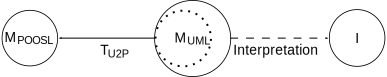
\includegraphics[scale=0.7]{introduction/figs/uml-to-poosl}
 \caption{Envisioned outcome of the Ideals project}
 \label{fig:introduction:ideals}
\end{figure}

Figure~\ref{fig:introduction:ideals} schematically depicts the desired outcome of the part of the Ideals project that concerned MDSE.
It shows that information is distilled from a large \UML model~\Model{UML} and transformed to a \POOSL model~\Model{POOSL} by means of a model transformation~\Transformation{U2P}.
The dotted circle illustrates that only a part of the information contained in the \UML model is used to create the \POOSL model.
The primary purpose of model~\Model{UML} is to serve as the design of an implementation~\Implementation{} of a system.
Software engineers interpret model~\Model{UML} and develop implementation~\Implementation{} manually, as depicted by the dashed arrow.

While developing the transformation from \UML to \POOSL and experimenting with the creation of suitable \UML models, a number of problems surfaced.
The diagrams of the \UML are not necessarily complete or consistent~\cite{Lange04anempirical, Lange03anempirical}, and its lack of formal semantics gives rise to different interpretations of the constructs it offers.
The positive side of this is the freedom it offers its users, which is one possible explanation for the popularity of the language~\cite{Lange06}.
%%%Soukup and Soukup give another reason for the popularity of the \UML.
%%%They relate the popularity of graphical languages such as the \UML to the expressiveness of available programming paradigms~\cite{Soukup:2007:ICG:1300755.1301815}.
%%%Over time, software systems increase in size and complexity, and at some point, these systems have become too large to be conveniently expressed in languages that support the prevalent programming paradigms.
%%%To bridle the complexity of the systems they develop, software engineers then turn to graphical languages.
%%%According to Schmidt, the growing complexity of software systems is also an explanation for the rising popularity of MDSE~\cite{Schmidt2006}.
Although \UML models are allowed to be inconsistent and incomplete, however, models that are the starting point for a transformation to \POOSL need to be consistent and complete.
This requirement gives rise to very elaborate \UML models, and creating such models using commercially available graphical editors proved to be cumbersome.
Furthermore, the constructs of the \UML were not adequate for describing models suited for performance analysis.
The language does not offer the appropriate abstractions for all aspects of the desired performance model, and some of the constructs offered by \POOSL had no equivalent counterpart in the \UML.

When the Ideals project was finished, we decided to create a new DSML to replace the \UML as a starting point for the transformation to \POOSL because of the aforementioned difficulties.
Additionally, this newly developed DSML was intended to be a suitable starting point for transformations to other formalisms and to have an intuitive graphical syntax similar to that of the \UML.
We named this DSML the Simple Language of Communicating Objects~(\SLCO).
Inspired by the Falcon project~\cite{Falcon2011}, we decided to use a small system of interoperating conveyor belts as a case study for \SLCO.
The overall challenge of the Falcon project was developing a fully integrated and automated logistics warehouse of the future.
Conveyor belts form an important part of such a warehouse.
Another goal for our DSML thus became to automatically generate software for the controllers of such conveyor belts, based on high-level descriptions specified in the DSML.
For verification of \SLCO models by means of model checking~\cite{Clarke1999}, we decided to develop a transformation to \Promela, the specification language of the model checker~\Spin~\cite{Holzmann2003}.

\begin{figure}[hbt]
 \centering
 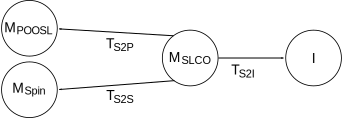
\includegraphics[scale=0.7]{introduction/figs/dsml-to-poosl}
 \caption{A single \SLCO model for code generation and formal analysis}
 \label{fig:introduction:dsml-to-poosl}
\end{figure}

Figure~\ref{fig:introduction:dsml-to-poosl} schematically depicts the automated generation of a model~\Model{POOSL} for performance analysis, a model~\Model{Spin} for verification, and an implementation~\Implementation{} for a system of interoperating conveyor belts from a model~\Model{SLCO} specified using the newly developed DSML.
The models for formal analysis and the implementation are generated by means of the model transformations~\Transformation{S2P}, \Transformation{S2S}, and~\Transformation{S2I}.
%The fact that model~\Model{SLCO} contains less superfluous information compared to model~\Model{UML} is indicated by its size.

The development of \SLCO and its accompanying model transformations was also triggered by the desire to investigate the internal and external quality of model transformations.
The quality of the definition of a model transformation is referred to as the internal quality of a transformation, and the quality of the process of transforming a source model to a target model is referred to as the external quality of a model transformation~\cite{AmstelThesis2011}.
The research performed by Van Amstel mainly focuses on the internal quality of model transformations~\cite{AmstelThesis2011}, whereas the work described in this thesis is concerned with the external quality of model transformations and their correctness in particular.

To successfully develop the new DSML and the accompanying model transformations, a number of problems needed to be solved. 